%\tikzstyle{decision} = [diamond, draw, fill=blue!50]
\tikzstyle{line} = [draw, -stealth, thick]
%\tikzstyle{elli}=[draw, ellipse, fill=red!50,minimum height=8mm, text width=5em, text centered]
\tikzstyle{block1} = [draw, rectangle, fill=blue!03, text width=18mm, text centered, minimum height=5mm, node distance=0mm]
\tikzstyle{block2} = [draw, rectangle, fill=blue!10, text width=18mm, text centered, minimum height=5mm, node distance=0mm]
\tikzstyle{block3} = [draw, rectangle, fill=blue!20, text width=25mm, text centered, minimum height=5mm, node distance=0mm]
\singlespacing
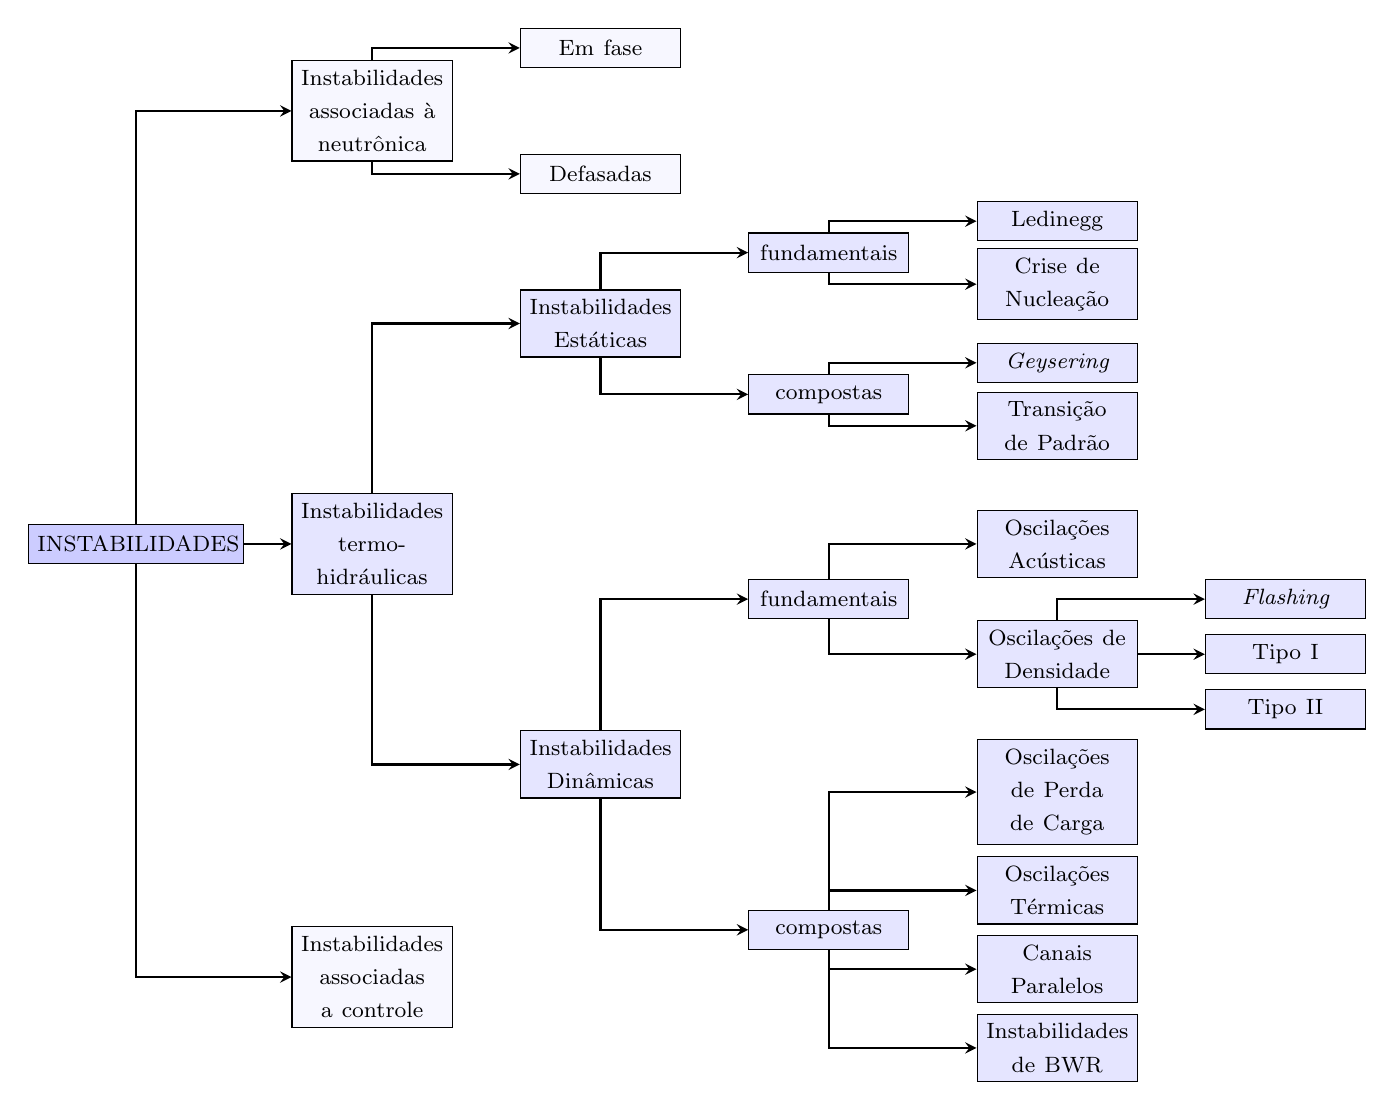
\begin{tikzpicture}
% primeiro nivel
\node [block3] (insta) {\footnotesize{INSTABILIDADES}};
% segundo nivel
\node [block2, right of=insta, xshift=30mm] (termo) {\footnotesize{Instabilidades termo-hidráulicas}};
\node [block1, right of=termo, yshift=55mm] (neutr) {\footnotesize{Instabilidades associadas à neutrônica}};
\node [block1, right of=termo, yshift=-55mm] (contr) {\footnotesize{Instabilidades associadas a controle}};
% terceiro nivel
\node [block2, right of=termo, xshift=29mm, yshift=28mm] (estat) {\footnotesize{Instabilidades Estáticas}};
\node [block2, right of=termo, xshift=29mm, yshift=-28mm] (dinam) {\footnotesize{Instabilidades Dinâmicas}};
\node [block1, right of=neutr, xshift=29mm, yshift=8mm] (emfas) {\footnotesize{Em fase}};
\node [block1, right of=neutr, xshift=29mm, yshift=-8mm] (defas) {\footnotesize{Defasadas}};
% quarto nivel
\node [block2, right of=estat, xshift=29mm, yshift=9mm] (estaf) {\footnotesize{fundamentais}};
\node [block2, right of=estat, xshift=29mm, yshift=-9mm] (estac) {\footnotesize{compostas}};
\node [block2, right of=dinam, xshift=29mm, yshift=21mm] (dinaf) {\footnotesize{fundamentais}};
\node [block2, right of=dinam, xshift=29mm, yshift=-21mm] (dinac) {\footnotesize{compostas}};
% quinto nivel
\node [block2, right of=estaf, xshift=29mm, yshift=4mm] (ledin) {\footnotesize{Ledinegg}};
\node [block2, right of=estaf, xshift=29mm, yshift=-4mm] (crise) {\footnotesize{Crise de Nucleação}};
\node [block2, right of=estac, xshift=29mm, yshift=4mm] (geyse) {\footnotesize{\it Geysering}};
\node [block2, right of=estac, xshift=29mm, yshift=-4mm] (padra) {\footnotesize{Transição de Padrão}};
\node [block2, right of=dinaf, xshift=29mm, yshift=7mm] (acust) {\footnotesize{Oscilações Acústicas}};
\node [block2, right of=dinaf, xshift=29mm, yshift=-7mm] (densi) {\footnotesize{Oscilações de Densidade}};
\node [block2, right of=dinac, xshift=29mm, yshift=17.5mm] (perda) {\footnotesize{Oscilações de Perda de Carga}};
\node [block2, right of=dinac, xshift=29mm, yshift=5mm] (termi) {\footnotesize{Oscilações Térmicas}};
\node [block2, right of=dinac, xshift=29mm, yshift=-5mm] (paral) {\footnotesize{Canais Paralelos}};
\node [block2, right of=dinac, xshift=29mm, yshift=-15mm] (inbwr) {\footnotesize{Instabilidades de BWR}};
% sexto nivel
\node [block2, right of=densi, xshift=29mm, yshift=7mm] (flash) {\footnotesize{\it Flashing}};
\node [block2, right of=densi, xshift=29mm, yshift=0mm] (tipo1) {\footnotesize{Tipo I}};
\node [block2, right of=densi, xshift=29mm, yshift=-7mm] (tipo2) {\footnotesize{Tipo II}};
%arrows
% niveis 1-2
\path [line] (insta) |- (neutr);
\path [line] (insta) -- (termo);
\path [line] (insta) |- (contr);
% niveis 2-3
\path [line] (termo) |- (estat);
\path [line] (termo) |- (dinam);
\path [line] (neutr) |- (emfas);
\path [line] (neutr) |- (defas);
% niveis 3-4
\path [line] (estat) |- (estaf);
\path [line] (estat) |- (estac);
\path [line] (dinam) |- (dinaf);
\path [line] (dinam) |- (dinac);
% niveis 4-5
\path [line] (estaf) |- (ledin);
\path [line] (estaf) |- (crise);
\path [line] (estac) |- (geyse);
\path [line] (estac) |- (padra);
\path [line] (dinaf) |- (acust);
\path [line] (dinaf) |- (densi);
\path [line] (dinac) |- (perda);
\path [line] (dinac) |- (termi);
\path [line] (dinac) |- (paral);
\path [line] (dinac) |- (inbwr);
% niveis 5-6
\path [line] (densi) |- (flash);
\path [line] (densi) -- (tipo1);
\path [line] (densi) |- (tipo2);
%\path [line] (decision1) -| node[yshift=1mm, xshift=-10mm] {no} (process2); % exemplo de seta com texto
\end{tikzpicture}
\onehalfspacing
